\section{Method: Sweep-Valuation Attention}
\label{sec:method}

\Cref{fig:overview} summarises \SVF{}. An appearance backbone (CNN or ViT) produces patch tokens.
Two structural fields are derived from the same image: the \emph{blade}, a deterministic leaf mask,
and a \emph{learned venation field}, a vein-probability map predicted by a light head on early backbone
features. A directional sweep partitions the leaf into ordered slabs. For every direction--slab pair,
\SVA{} measures how much of each field's \emph{intrinsic volumes} (area and boundary length) enters
the filtration inside that slab, and uses \emph{the same slab} to restrict where the resulting token
attends among the patch tokens.

\begin{figure*}[t]
\centering
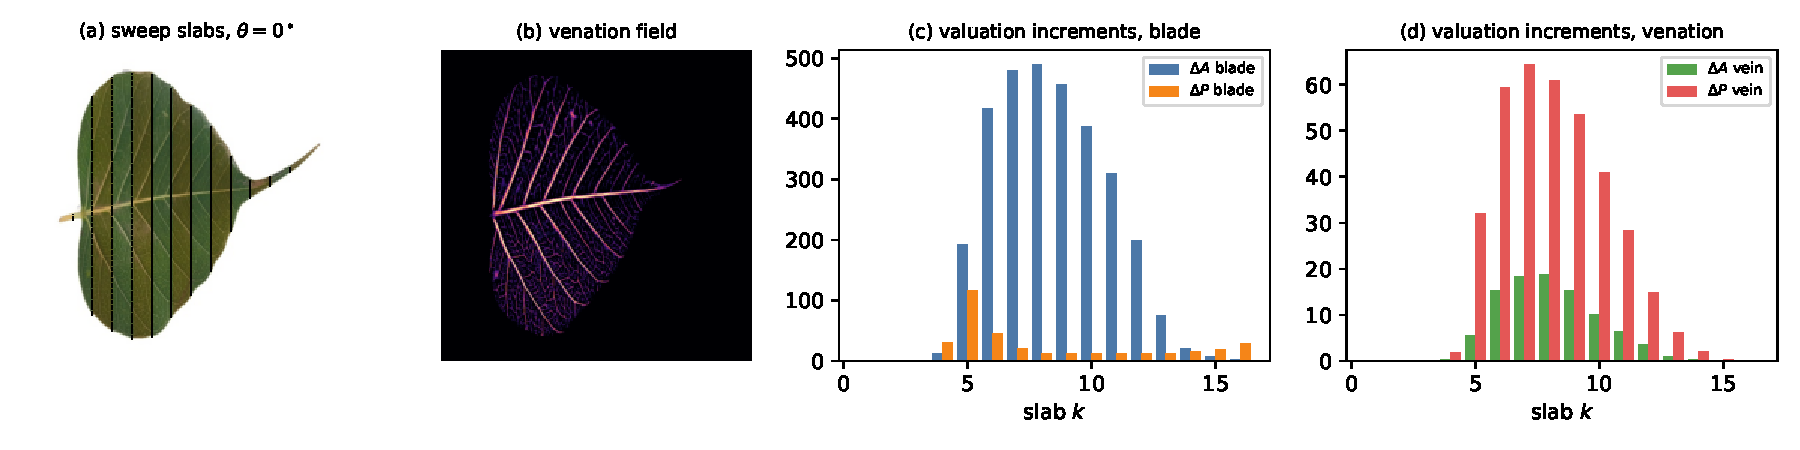
\includegraphics[width=\textwidth]{figures/fig_overview.pdf}
\caption{The sweep-valuation signal for one leaf (\textit{Ficus religiosa}) and one of the $K{=}32$
directions. (a)~The leaf is partitioned into $T{=}16$ slabs along $\theta$ in its centroid/RMS frame.
(b)~Ridge-filter vein pseudo-label that supervises the learned venation field. (c,d)~Area and
perimeter increments per slab for the blade and the venation field, shown here with unit weights; in
\SVA{} the cell weights are appearance-conditioned. Each slab's increments form the query of one
token, which attends to the image patches of the same slab. The long perimeter in the last blade
slabs comes from the drip tip.}
\label{fig:overview}
\end{figure*}
\subsection{Weighted cubical complexes}
The leaf crop is resampled to a $G\times G$ grid ($G{=}96$). Pixel centres $x_p$ are expressed in
a frame centred at the blade centroid and scaled by its root-mean-square radius, which makes all
quantities below invariant to translation and isotropic scale. We use the cubical complex whose
0-cells are pixels, whose 1-cells are pairs of 4-adjacent pixels and whose 2-cells are $2\times2$
pixel squares. Given per-pixel weights $a(p)\in[0,1]$, cells inherit the minimum weight of their
vertices,
\begin{equation}
  w_0(p)=a(p),\qquad w_1(e)=\min_{v\in e}a(v),\qquad w_2(q)=\min_{v\in q}a(v).
  \label{eq:weights}
\end{equation}
This keeps face monotonicity $w(\text{coface})\le w(\text{face})$, so the weighted complex is a fuzzy
subcomplex. For binary $a$ it reduces exactly to the standard cubical complex of the set.

\paragraph{Appearance-conditioned weights.} Two weight fields are built from mid-level backbone
features $f$ (bilinearly sampled at the grid), a small per-pixel MLP $g$ and a sigmoid $\sigma$:
\begin{equation}
 a_{\mathrm{b}}(p) = m(p)\,\sigma\!\big(g_{\mathrm{b}}(f(p))\big),\qquad
 a_{\mathrm{v}}(p) = m(p)\,v(p)\,\sigma\!\big(g_{\mathrm{v}}(f(p))\big),
\end{equation}
where $m$ is the blade mask and $v$ is the predicted vein probability. The last layer of $g$ is
initialised so that $a\approx 0.88\,m$ at the start of training. The vein head is pseudo-supervised
by a multiscale Sato ridge response~\citep{sato1998ridge} inside the eroded mask and also receives
task gradients through \SVA{}. In contrast to fixed intensity weights (WECT~\citep{cisewski2023wect}),
the weights are learned and conditioned on appearance. We stress that $a_{\mathrm{v}}$ is a
\emph{learned} venation field, not an observed vascular structure.

\subsection{Valuations of a weighted cubical complex}
Let $H_d=\sum_{c\in C_d}w_d(c)$ be the weighted number of $d$-cells. For a binary set the three
quantities
\begin{equation}
 A = H_2,\qquad P = 2H_1-4H_2,\qquad \chi = H_0-H_1+H_2
 \label{eq:valuations}
\end{equation}
are the area (number of unit squares), the boundary length in pixel units (every square contributes
four edges, and an edge shared by two squares is interior) and the Euler characteristic. They are
the cubical counterparts of the three planar intrinsic volumes. By Hadwiger's
theorem~\citep{hadwiger1957,klain1997}, every continuous, rigid-motion-invariant valuation on planar
convex bodies is a linear combination of these three. Because~\eqref{eq:valuations} is linear in the
cell weights, it extends directly to the fuzzy complex~\eqref{eq:weights}. Our proposed token uses
area and perimeter, i.e.\ the two \emph{metric} intrinsic volumes. The purely topological one, $\chi$,
is retained as an ablation (\cref{sec:abl}), because in our pilots it did not add information beyond
area and perimeter (\cref{sec:results}).

\subsection{Filtration increments along a sweep}
For a direction $\theta\in S^1$ we use the lower-star filtration,
$h_\theta(v)=\langle x_v,\theta\rangle$ and $h_\theta(c)=\max_{v\in c}h_\theta(v)$. Following the
sigmoid relaxation of DECT~\citep{roell2024dect}, a cell enters the filtration at threshold $t$ with
soft indicator $\sigma(\lambda(t-h_\theta(c)))$. Fix thresholds $t_0<t_1<\dots<t_T$, where
$t_1,\dots,t_{T-1}$ are uniform on $(-R,R)$, $t_0=-\infty$ and $t_T=+\infty$. The soft membership of
height $h$ in slab $k$ is
\begin{equation}
 s_k(h)=\sigma\big(\lambda(t_k-h)\big)-\sigma\big(\lambda(t_{k-1}-h)\big),\qquad k=1,\dots,T,
 \label{eq:slab}
\end{equation}
and because the outer thresholds are infinite, $\sum_k s_k(h)=1$ for every $h$. The
\emph{filtration increment} of the weighted $d$-cell count in slab $k$ is
$\Delta H_d(\theta,k)=\sum_{c\in C_d}w_d(c)\,s_k(h_\theta(c))$, and the valuation increments follow by
linearity:
\begin{equation}
 \Delta A(\theta,k)=\Delta H_2,\qquad \Delta P(\theta,k)=2\Delta H_1-4\Delta H_2,\qquad
 \dchi(\theta,k)=\Delta H_0-\Delta H_1+\Delta H_2 .
 \label{eq:increment}
\end{equation}
Each is the change of the corresponding relaxed valuation of the sublevel set between $t_{k-1}$ and
$t_k$, and $\sum_k$ telescopes to the total valuation of the leaf, independently of $\theta$. We
compute~\eqref{eq:increment} for the blade ($a_{\mathrm b}$) and the venation field ($a_{\mathrm v}$)
with $K$ uniform directions and $T$ slabs ($K{=}32$, $T{=}16$, $R{=}2$, $\lambda=\kappa T/2R$ with
$\kappa{=}4$).

\paragraph{Sweep-valuation token.} The structural feature of token $(\theta,k)$ is the 8-vector of
area and perimeter increments of both fields together with their cumulative values up to slab $k$,
\begin{equation}
 \phi(\theta,k)=\operatorname{slog}\Big[\Delta A_{\mathrm b},\Delta P_{\mathrm b},\Delta A_{\mathrm v},
 \Delta P_{\mathrm v},\ \textstyle\sum_{j\le k}(\cdot)\Big],\qquad \operatorname{slog}(x)=\operatorname{sign}(x)\log(1+|x|).
\end{equation}
The increments describe the local width profile and boundary complexity of the slab; the cumulative
values locate it within the leaf. The Euler variant replaces $\phi$ by
$[\dchi_{\mathrm b},\dchi_{\mathrm v},\chi_{\mathrm b}(t_k),\chi_{\mathrm v}(t_k)]$, and the Hadwiger
variant uses all three valuations (12 features).

\paragraph{Efficient computation.} Directions are fixed and coordinates come from the mask, so the
heights carry no gradient; only the weights do. We hard-bin heights into $n_b{=}256$ fine bins,
scatter-add cell weights per dimension into a per-direction histogram, and apply the slab
kernel~\eqref{eq:slab} evaluated at bin centres with one matrix product (the kernel is built in
double precision). This costs $O(BKN)$ memory for $N$ cells, needs no sorting, and is exact in the
telescoping and sharp limits (verified by unit tests, \cref{app:tests}).

\subsection{Co-registered slab attention}
Each direction--slab pair $(\theta,k)$ defines one sweep token with query
$q_{\theta k}=\mathrm{MLP}(\phi(\theta,k))+e_k$, where $e_k$ is a learned slab-index embedding. The token
cross-attends to the backbone patch tokens $\{z_p\}$ with an additive bias derived from the
\emph{same} soft slab membership~\eqref{eq:slab}, evaluated at patch centres:
\begin{equation}
 \mathrm{attn}_{(\theta,k)}(p)\propto\exp\!\Big(\tfrac{\langle W_Q q_{\theta k},\,W_K z_p\rangle}{\sqrt{d}}
 +\log\!\big(s_k(\langle x_p,\theta\rangle)\,\bar m(p)+\epsilon\big)\Big),
 \label{eq:attn}
\end{equation}
where $\bar m(p)$ is the fraction of leaf pixels in patch $p$ and $\epsilon=10^{-4}$. The structural
measurement and the visual evidence attached to it are thus taken over the same filtration-defined
region. To the best of our knowledge, we did not find prior work that explicitly co-registers
filtration-derived valuation increments with attention restricted to the corresponding filtration
slab (\cref{sec:related}). The attention output is added to the query with a mass gate
$M/(M+0.5)$, $M=\sum_p s_k\bar m$, so that slabs outside the leaf contribute little. The $KT{=}512$
tokens are mixed by a two-layer \emph{sweep transformer} whose learned relative position bias depends
only on $(\Delta\theta \bmod K,\Delta k)$. Tokens are mean-pooled and concatenated with the backbone's
global token for classification. Training minimises cross-entropy (label smoothing $0.1$) plus
$0.2\times$ the masked BCE of the vein head.

\subsection{Symmetry properties}
\begin{proposition}\label{prop:equiv}
Let $\mathcal R$ be a rotation by a multiple of $90^\circ$ acting on the pixel grid and let the
weights be unit (binary blade). Then $\Delta A$, $\Delta P$ and $\dchi$ of $\mathcal R I$ equal
those of $I$ cyclically shifted by $K/4$ along $\theta$ for each multiple of $90^\circ$; for
rotations by $2\pi/K$ the same holds up to grid resampling.
\end{proposition}
\noindent The proof follows from $\langle \mathcal R x,\theta\rangle=\langle x,\mathcal R^{-1}\theta\rangle$,
the equivariance of the centroid/RMS frame, and the fact that a $90^\circ$ grid rotation maps cells
of each dimension bijectively onto cells of the same dimension (so the counts $H_d$ in every slab are
permuted, not changed). It is checked numerically in \cref{app:tests}. The appearance-conditioned
weighted signal and the full \SVF{} inherit the rotation behaviour of the backbone
($f(\mathcal R I)\neq\mathcal R f(I)$ in general). We therefore do \emph{not} claim exact invariance
for them and evaluate their behaviour empirically (\cref{sec:results}). Rotation-equivariant
ECT tokenisation as such is not our contribution~\citep{blaser2026encoding}.

\subsection{Controls built from the same code}
\label{sec:controls}
To isolate what matters, we compare five models that share the backbone, vein head, training recipe
and, where applicable, the token width and transformer depth:
\begin{enumerate}
 \item \textbf{plain}: backbone global token only;
 \item \textbf{global}: the full $K\times T\times8$ valuation grid flattened through an MLP and fused
   globally (in the spirit of~\citep{phgnet2023,gu2026multifiltration}); same structural content,
   no co-registration;
 \item \textbf{strip}: strip pooling~\citep{hou2020strip}, i.e.\ mask-weighted means of patch tokens
   over every row and column of the patch grid, with learned positions and the same two-layer
   transformer; localised directional pooling without an object-centred sweep or structural content;
 \item \textbf{slab-only}: identical to \SVA{} except that $\phi\equiv0$, so each query is only the slab
   embedding $e_k$; the same co-registered slab geometry, no valuation content;
 \item \textbf{\SVA{}} (proposed).
\end{enumerate}
Model 2 versus 5 asks whether co-registration matters; 3 versus 5 asks whether an object-centred
filtration sweep matters beyond generic directional pooling; 4 versus 5 asks whether the measured
valuations matter beyond the slab geometry itself.
